\chapter{Electron energy scale and resolution corrections}
\label{app:electron_enenergy_scale_corr}

The cumulative impact of the electron reconstruction process (summarised in Eqn~\ref{eqn:egamma_reco_energy}), including application of the electron energy scale and resolution corrections, is shown in Figure~\ref{fig:cms_energy_corrs}, for electrons from \Zee decays. 

\begin{figure}[htbp!]
\centering
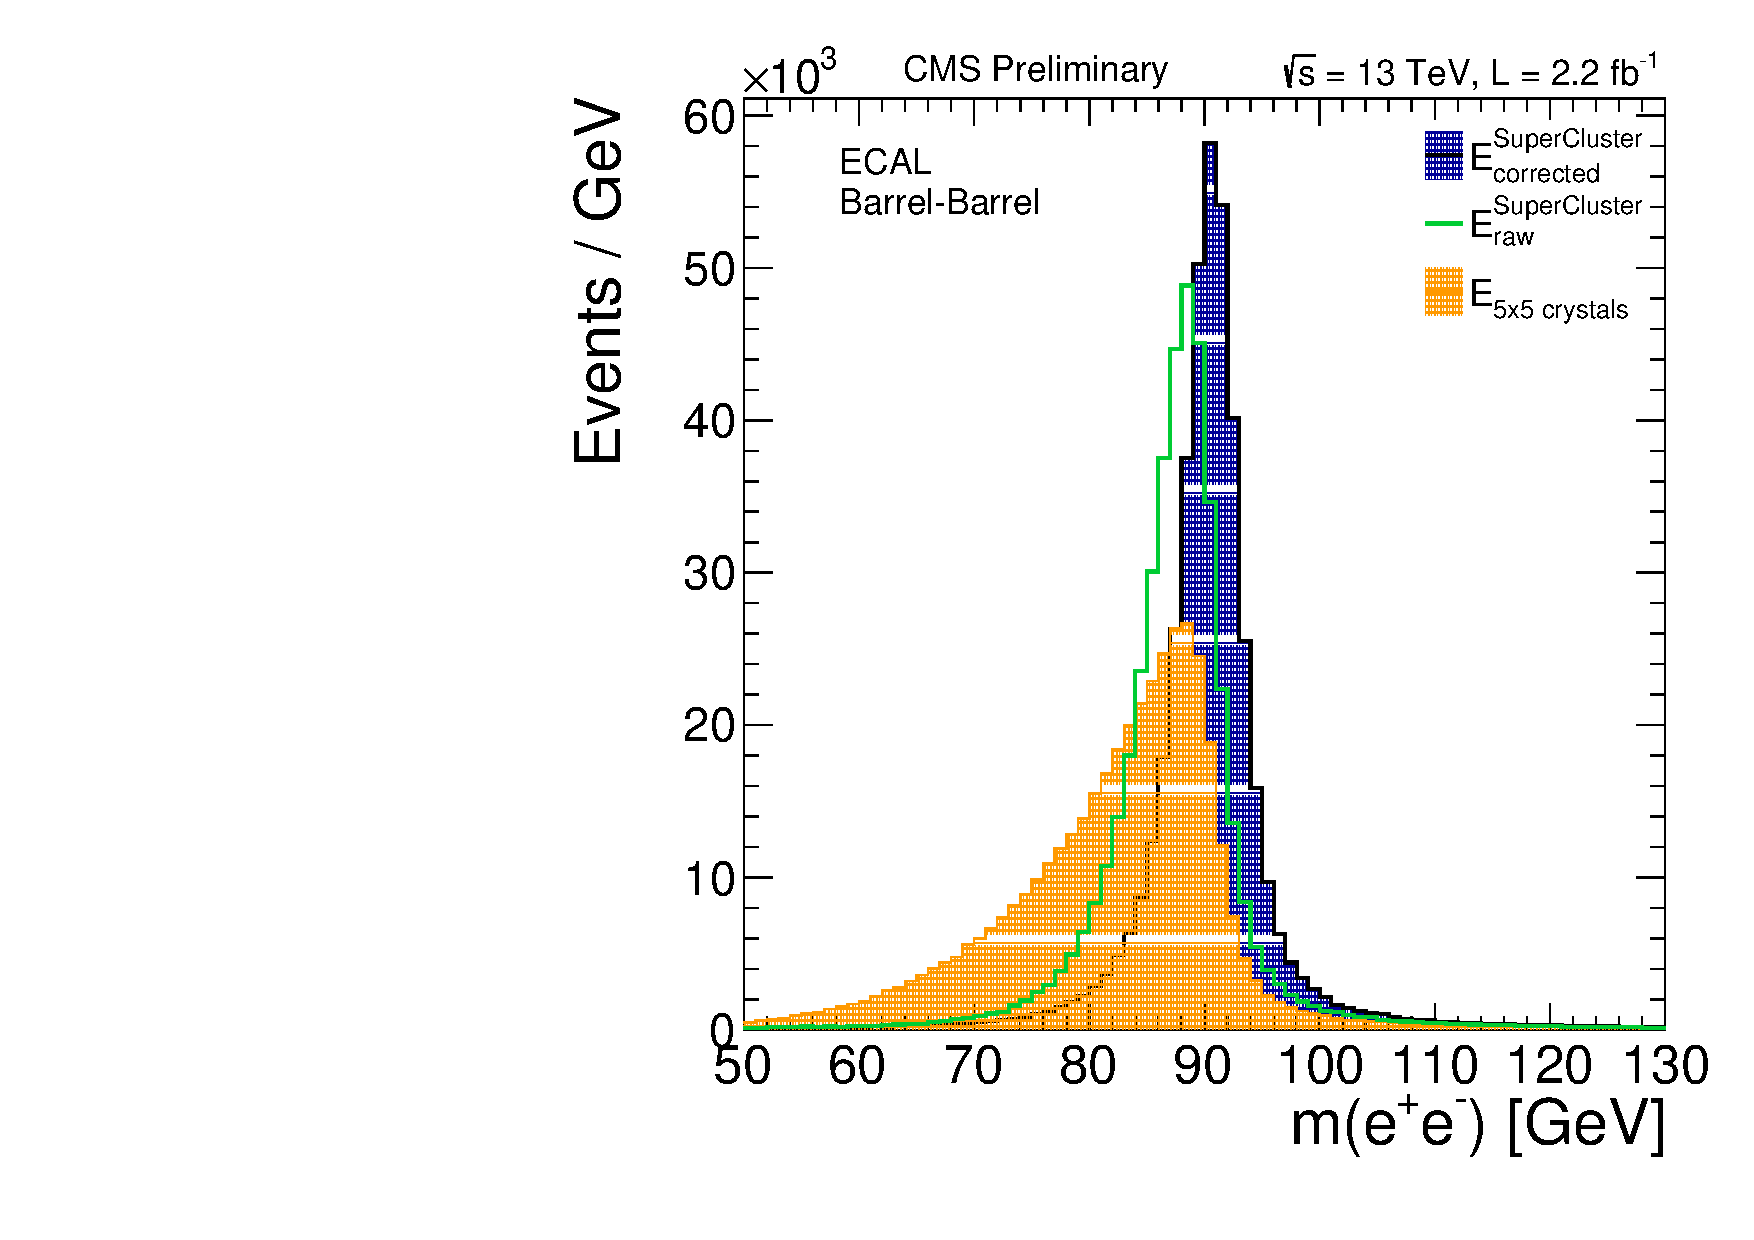
\includegraphics[width =0.5\linewidth]{Figures/Hee/simulationCorrections/DY/energy_scale_corrs_breakdown_EB.pdf}\hfill%
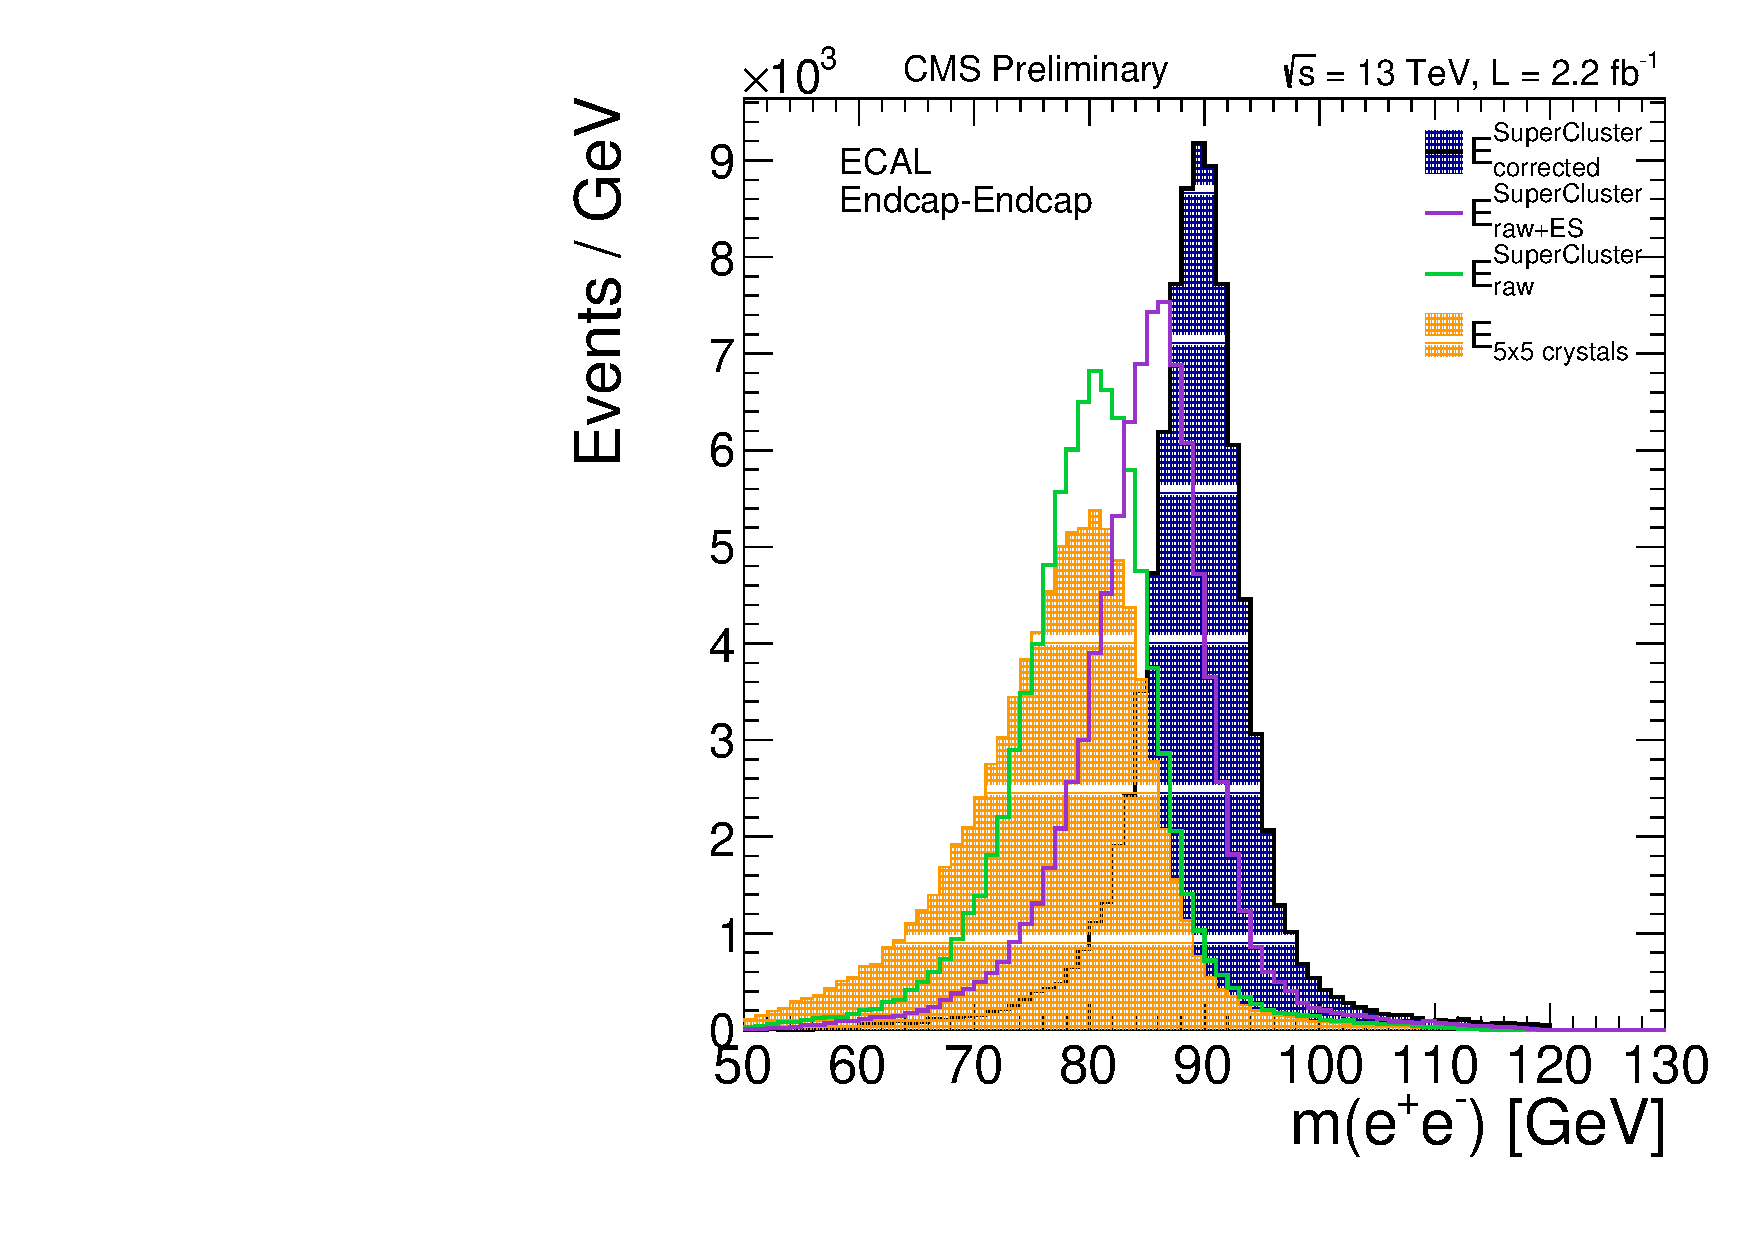
\includegraphics[width =0.5\linewidth]{Figures/Hee/simulationCorrections/DY/energy_scale_corrs_breakdown_EE.pdf}\hfill
\caption[The impact of electron energy scale and resolution corrections for electrons from \Zee decays.]{The invariant mass of electrons from \Zee decays, shown at different stages of the electron reconstruction process, including application of the electron energy scale and resolution corrections. Electrons reconstructed in the EB (EE) region are shown in the left (right) plot. The data shown were collected during the 2015 period of the LHC operation. Each stage in the reconstruction is compared to a simple energy sum of the $5\times5$ array of ECAL crystals centred on the electron candidate, the distribution for which is shown in yellow. Following the clustering process, the invariant mass determined using the electron supercluster properties is shown in the green histogram. For electrons reconstructed in the endcap, the invariant mass computed using the combination of the supercluster energy and the energy deposited in the ES is shown by the purple histogram. The final invariant mass distribution, following the application of the electron energy scale and resolution corrections, is shown in the blue histogram. Figure taken from Ref~\cite{Electron_energy_scale_cumulative}.}
\label{fig:cms_energy_corrs}                                              
\end{figure}
